\documentclass[times, twocolumn]{article}
\usepackage{graphicx} % Required for inserting images
\usepackage{subcaption}
\usepackage{amsmath}
\usepackage{float}
\usepackage{pgfplots}
\usepackage{subcaption}
\usepackage{comment}
\usepackage[a4paper, total={7in, 9in}]{geometry}
\usepackage{biblatex}

\addbibresource{mybib.bib}

\title{Spotify Tracks Genre Classification}
\author{Nabeha Barkatullah, Mia Striebeck, Laksha Karthikeyan, Carson Chiem, Shuzo Naruse}
\date{May 20, 2024}

\begin{document}
\maketitle

\newpage
% abstract
\begin{abstract}
Discovering new music that fits within your music taste is time-consuming and difficult. On top of there being an abundance of music to sift through, finding songs from the bulk that you actually enjoy listening to can go either way. With this project, we aim to utilize a Spotify dataset to build a model to classify songs under genres, with the potential of being part of a song recommendation system. Using the attributes from the dataset, such as the relevant music listening patterns and classification of songs, we will predict the genre a song falls under. Our goal is to build a classification model that predicts a song’s genre based on user-inputted track features.
\end{abstract}
\section{Introduction}
[include intro]
% background
\section{Background}
%literature review
\section{Literature Review}
\newpage
\section{Dataset Description and EDA}
\subsection{Dataset Description}
The selected Kaggle dataset contains data on Spotify songs from over 125 genres, with each song having associated features related to identification of each track, audio characteristics, or popularity and genre classifications. The original set contained around 114k data points (songs) condensed in a CSV format, with 20 features, which are track id, artist name, album name, track name, popularity, duration (ms), explicit, danceability, energy, key, loudness, mode, speechiness, acousticness, instrumentalness, liveness, valence, tempo, and time signature. Popularity is the ranking of each song on a scale of 1 to 100, duration of the track is in milliseconds (ms), explicit indicates if a song contains explicit lyrics or not, represented respectively as true or false, danceability is a measure, from 0 to 1, of how a song is considered appropriate for dancing, energy is a measure, from 0 to 1, of intensity, key is in regards to overall musical pitch, loudness is measured overall in decibels (dB), mode indicates if the track is on a major or minor scale (1 or 0), speechiness measures, from 0 to 1, the level of spoken words in a track, acousticness is a measure, from 0 to 1, of instruments used without electrical amplification, instrumentalness is a measure, from 0 to 1, of a track containing vocals, liveness is the likelihood of a song being performed in front of an audience, valence measures the interpretation of a song as positive or negative, tempo is the speed of a track, measured in beats per minute (BPM), and time signature indicates the number of beats in each measure of the piece. All are continuous variables, except for track id, artist name, album name, track name, explicit, popularity and track genre, which are categorical. Popularity in particular is ordinal categorical, as tracks are assigned a ranking of popularity. 

In pre-processing the data, we checked for duplicate rows and missing values. 32,656 rows were dropped, as they were each identified as having the same track name and artist as an another track. The remaining rows of distinct tracks were filtered to identify missing values for each feature, which identified one track having 3 missing values. Furthermore, the genre feature in the original dataset contained 125 categories, however, as many genres were more specific sub-genres, we grouped these sub-genres under their respective overall genres. For instance, tracks with the sub-genres "emo," "punk," and "garage," were all re-classified under the genre "punk-rock." This allowed for greater accuracy of genre classification, with reduced complexity and risk of overfitting, as the model would be less likely to fit too closely to the data of these more specific sub-genres which also have small sample sizes. The dataset was ultimately filtered to only contain the 10 most popular genres, removing the rows of all other genres. Thus, as the duplicate rows, the one row with a missing value and the rows not a part of the top 10 genres were dropped, the resulting cleaned dataset contained 81,344 rows of distinct tracks.
\subsection{Exploratory Data Analysis}
As shown in Figure \ref{graph:dists}, the danceability and tempo have nearly normal distributions. The distribution of loudness is left-skewed while acousticness, speechiness, liveliness are right-skewed. This signifies that while most of the songs in this dataset are moderately loud, there are some that have particularly low levels of loudness, that makes the distribution skew to the right. Similarly, acousticness, speechiness and liveliness For popularity, if the songs with the value 0 are taken out, the distribution would almost be normal. Also, energy has an increasing distribution.
% adding Figure 1 - image of feature distributions
\begin{figure}[H]
    \centering
    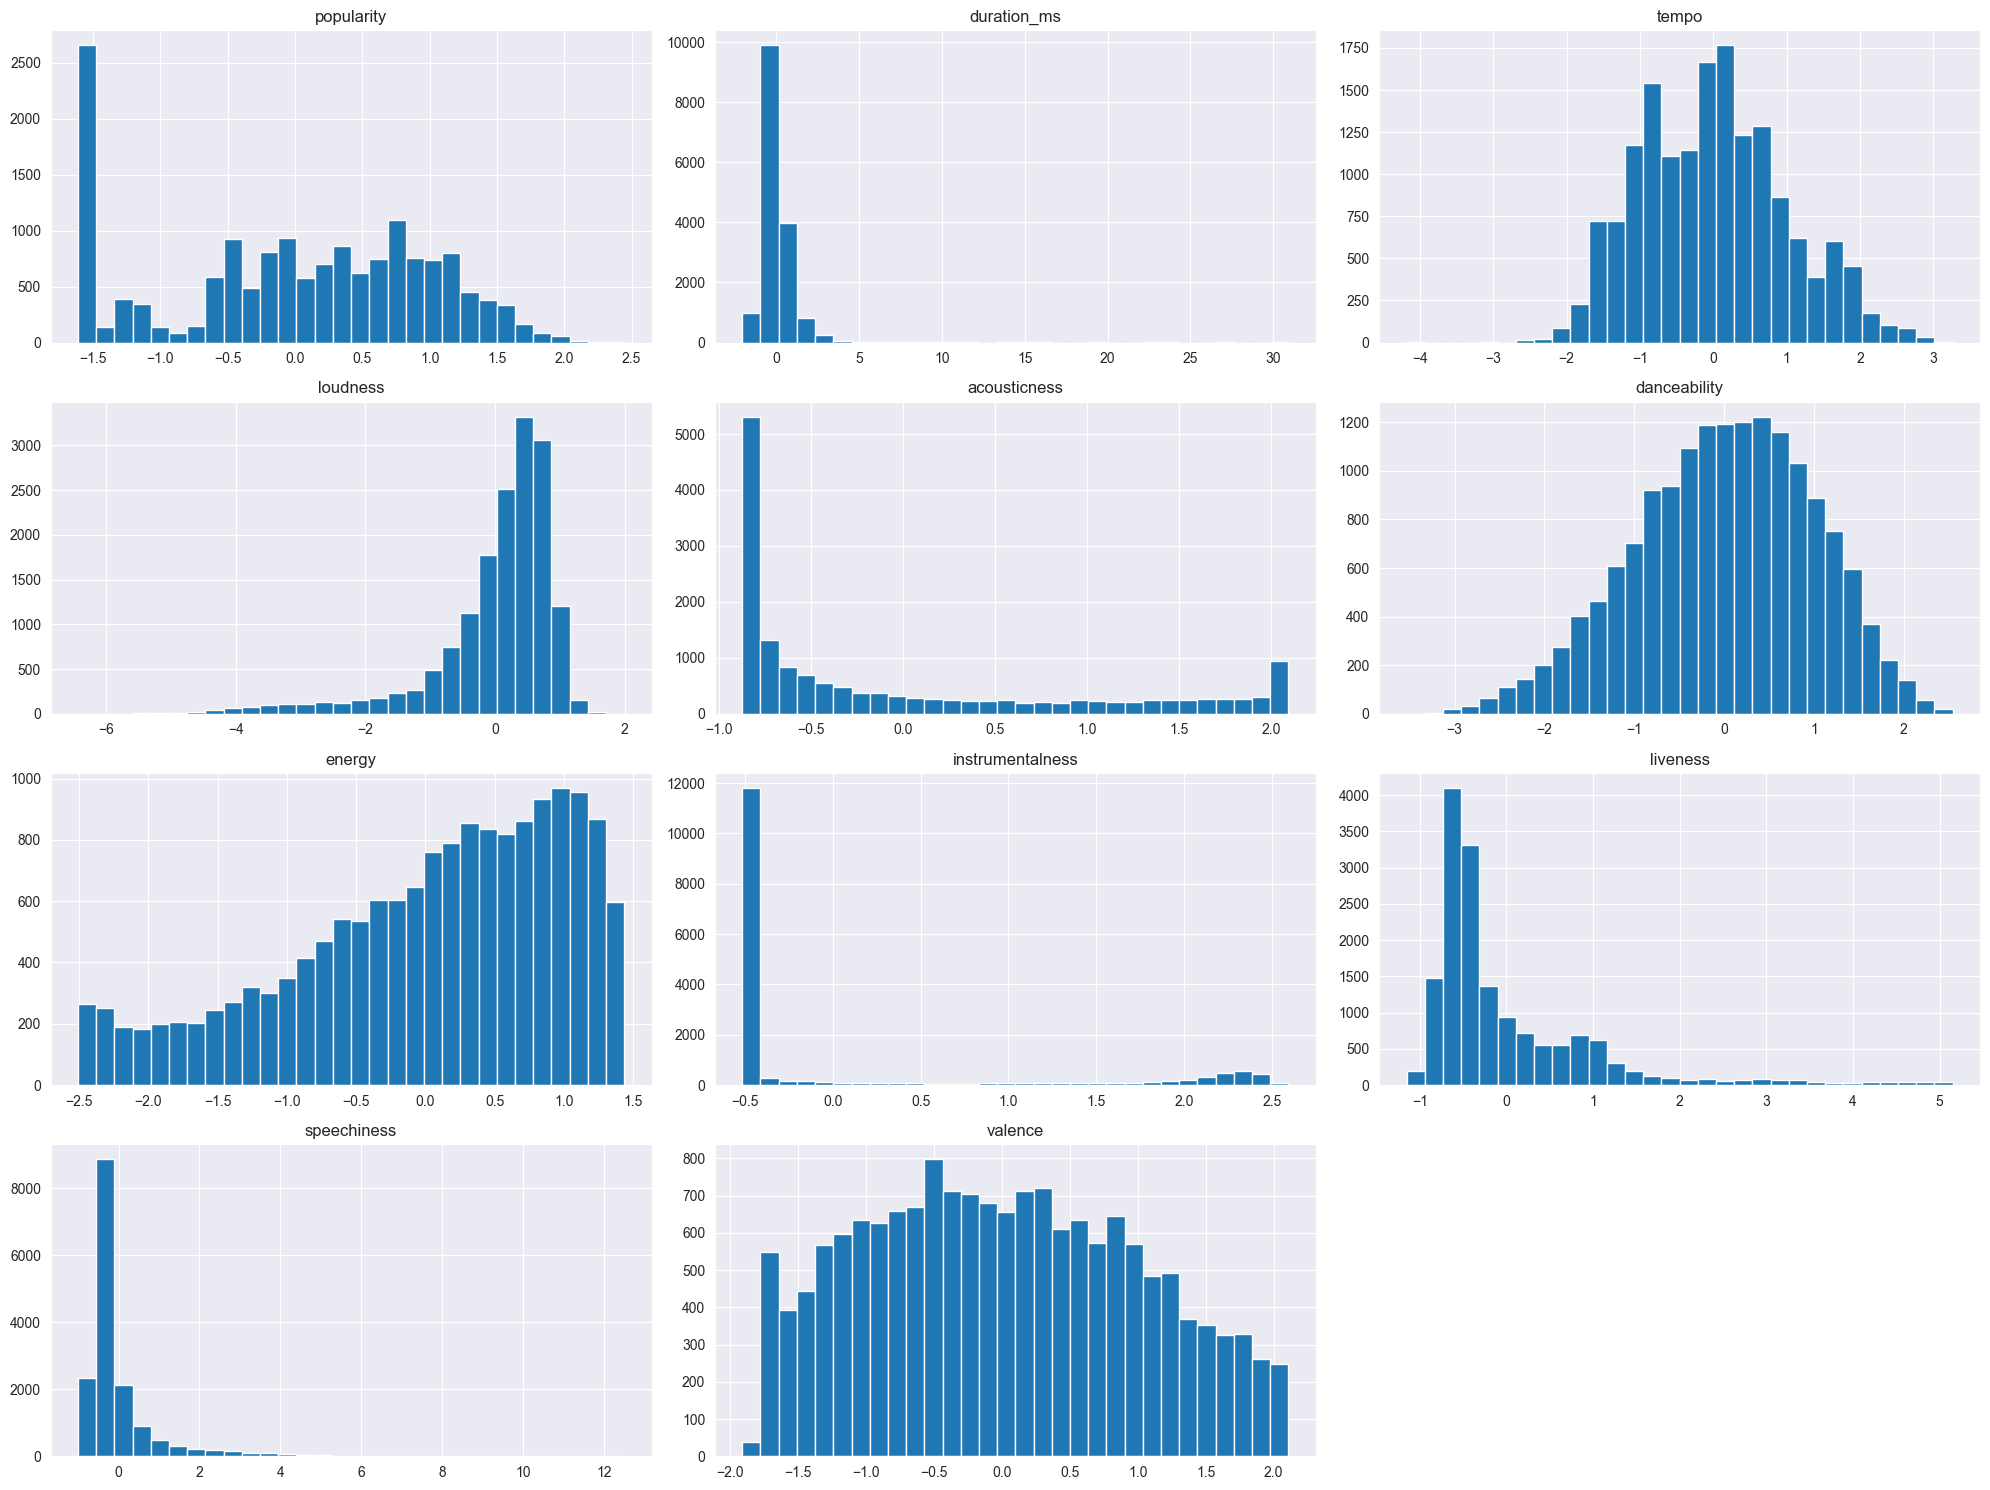
\includegraphics[width=0.55\textwidth]{feature_dists.png}
    \caption{Caption}
    \label{graph:dists}
\end{figure}

% adding Figure 2 - boxplots
\begin{figure}[H]
    \centering
    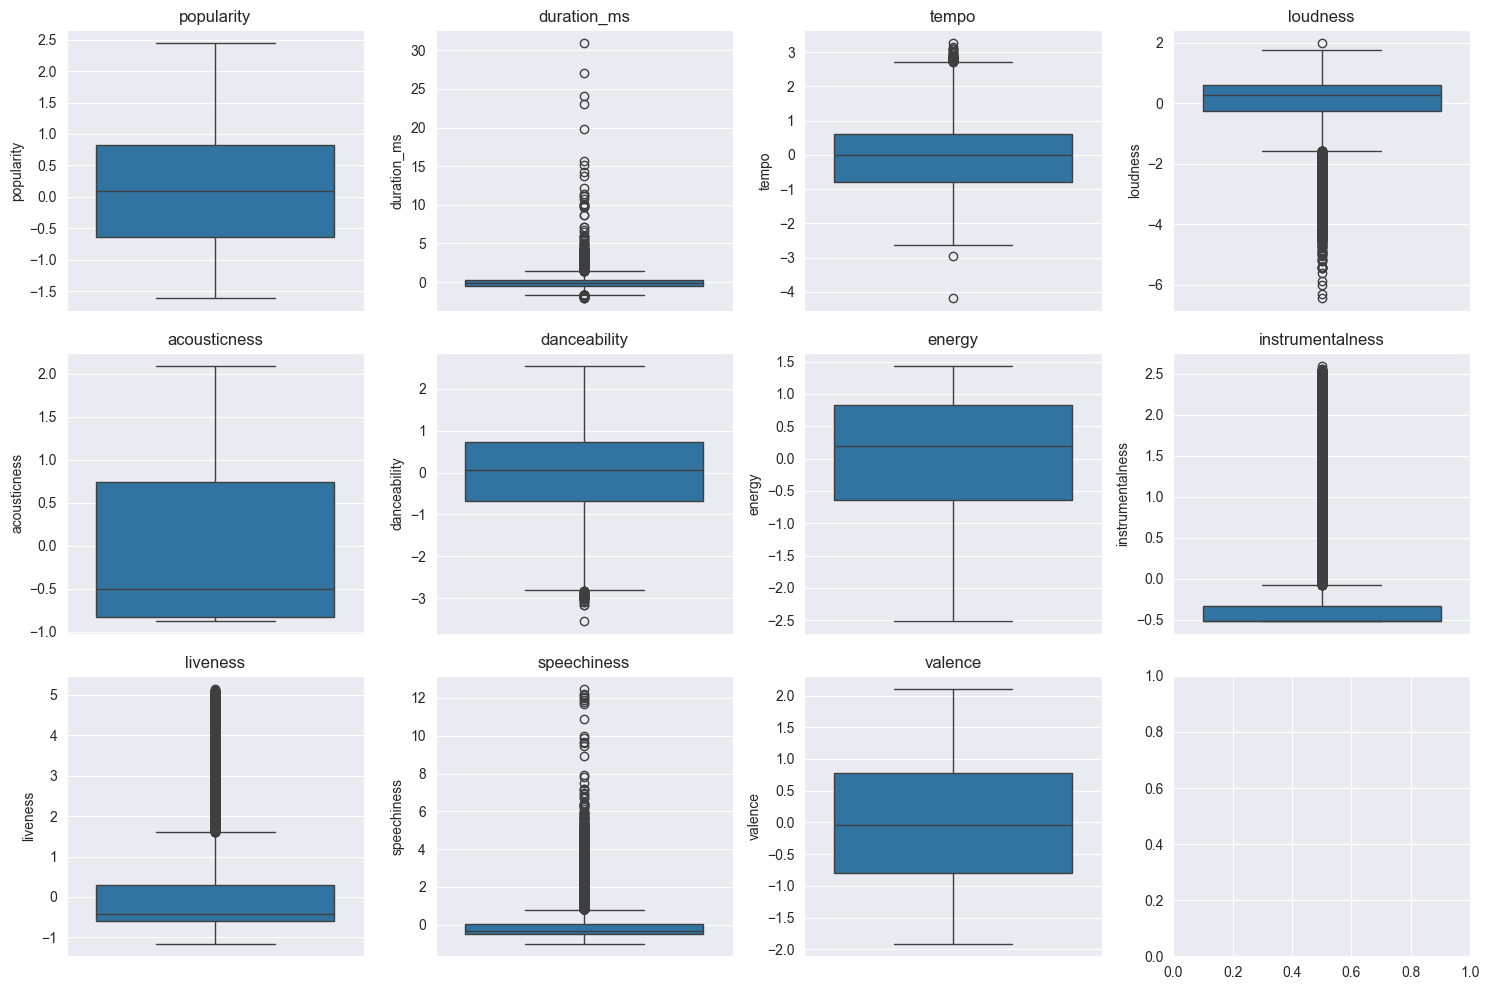
\includegraphics[width=0.5\textwidth]{feat_boxplots.png}
    \caption{Caption}
    \label{Boxplots}
\end{figure}

Box plots were also used to visualize skewed data and identify outliers. The box plots in Figure \ref{Boxplots} map the distributions for the ordinal categorical predictor variable popularity, and all the continuous predictor variables, duration, tempo, loudness, acousticness, danceability, energy, instrumentalness, liveliness, speechiness and valence. From this visualization, it is evident that acousticness, energy and valence have no outliers, while the other features do. The presence of outliers is reasonable as it merely shows the diversity of the songs in our dataset, and ultimately, the variety in levels of these features is what characterizes the different music styles that allow a song to be categorized under a certain genre.

It's also good to note the absence of outliers, as the presence of outliers may cause problems during model fitting. Since our data is clean, we can better avoid inflated error metrics that can significantly impact model performance by skewing parameter estimates.

In addition to understanding the correlations between the features and music genre or idk, it's important to understand the correlations \textit{between} the features in building accurate models. Correlations between features provide insights into how the variables in the dataset interact with each other, which can guide feature selection, model construction, and interpretation of results. While strong correlations between features may indicate redundancy or multicollinearity*, leading to potential model instability or overfitting, they can also highlight important relationships that contribute to the predictive power of the model. Therefore, it is essential to examine the feature correlations for making informed decisions about whether to keep or remove features based on the specific context of the ML problem and the goals of the analysis.\\

\begin{figure}[H]
    \centering
    \textbf{Pearson's Correlation Heatmap of Relevant Features}
    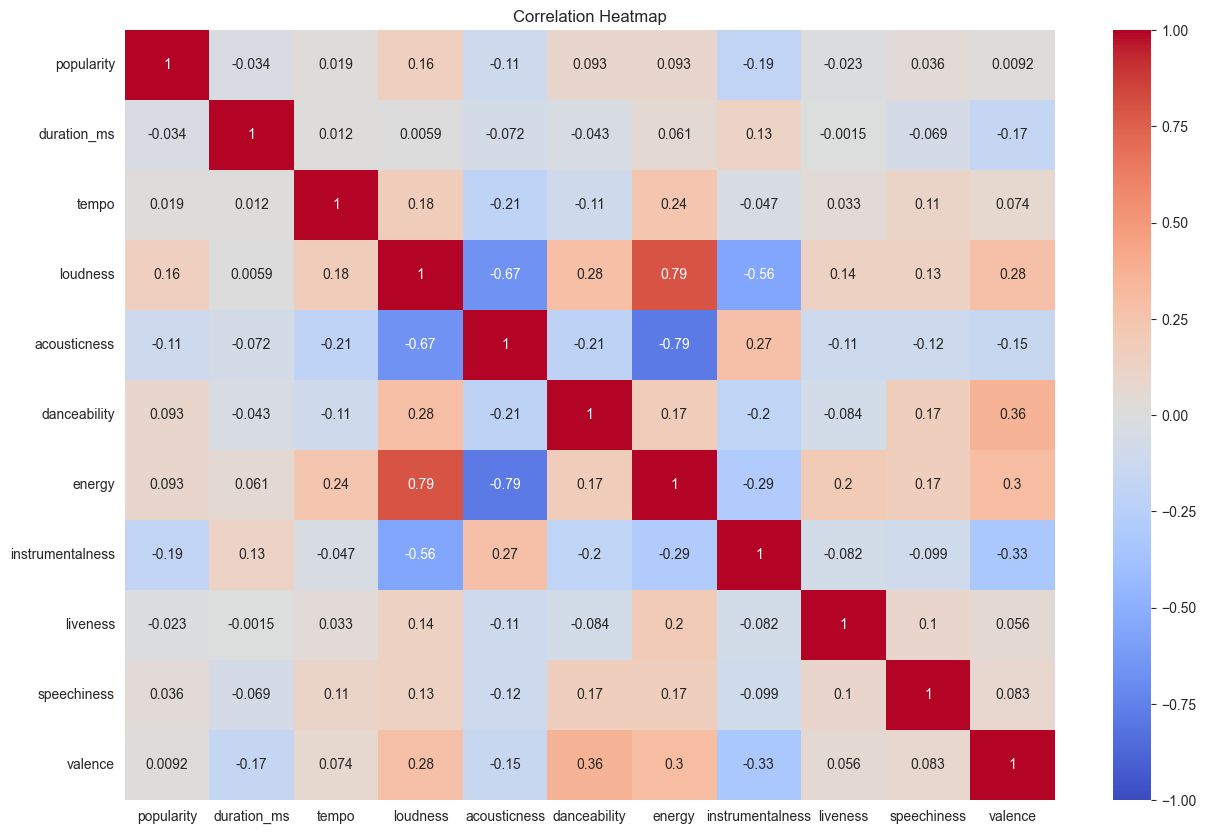
\includegraphics[width=1.0\linewidth]{corr_heatmap.png}
    \caption{The Pearson's correlation heatmap depicts the pairwise correlations between the 11 features that are relevant to the characteristics of each track. Each cell in the heatmap represents the correlation coefficient between two features, ranging from -1 to 1. A value close to 1 indicates a strong positive correlation, while a value close to -1 suggests a strong negative correlation. A correlation of 0 indicates no linear relationship between the features. This heatmap provides insights into the interplay between different features, guiding feature selection and model interpretation.}
    \label{heatmap}
\end{figure}

Despite observing both weak and strong correlations among the 13 features in Figure \ref{heatmap}, words.

\section{Proposed Methodology}
In order to build a classification model to classify the genre of a track based on the predictor variables related to audio characteristics, our modeling approach entailed identifying techniques that would work well for multi-class classification, as our dataset contains multiple possible genres. We examined the performance of K-nearest neighbors clustering and Random Forest models.

\section{Experimental Results and Evaluation}
\subsection{Model Performances}

\subsection{Model Implications}

\section{Conclusion}

\section{Discussion}

\section{Github link and Project Roadmap}

\section{Works Cited}
\printbibliography


\end{document}
